\documentclass[border=10pt]{standalone}

\usepackage{tikz}
\usepackage{tikzsymbols}
\usetikzlibrary{calc,patterns,shapes.geometric}

\def\centerarc[#1](#2)(#3:#4:#5){\draw[#1] ($(#2)+({#5*cos(#3)},{#5*sin(#3)})$) arc (#3:#4:#5);}

\begin{document}
	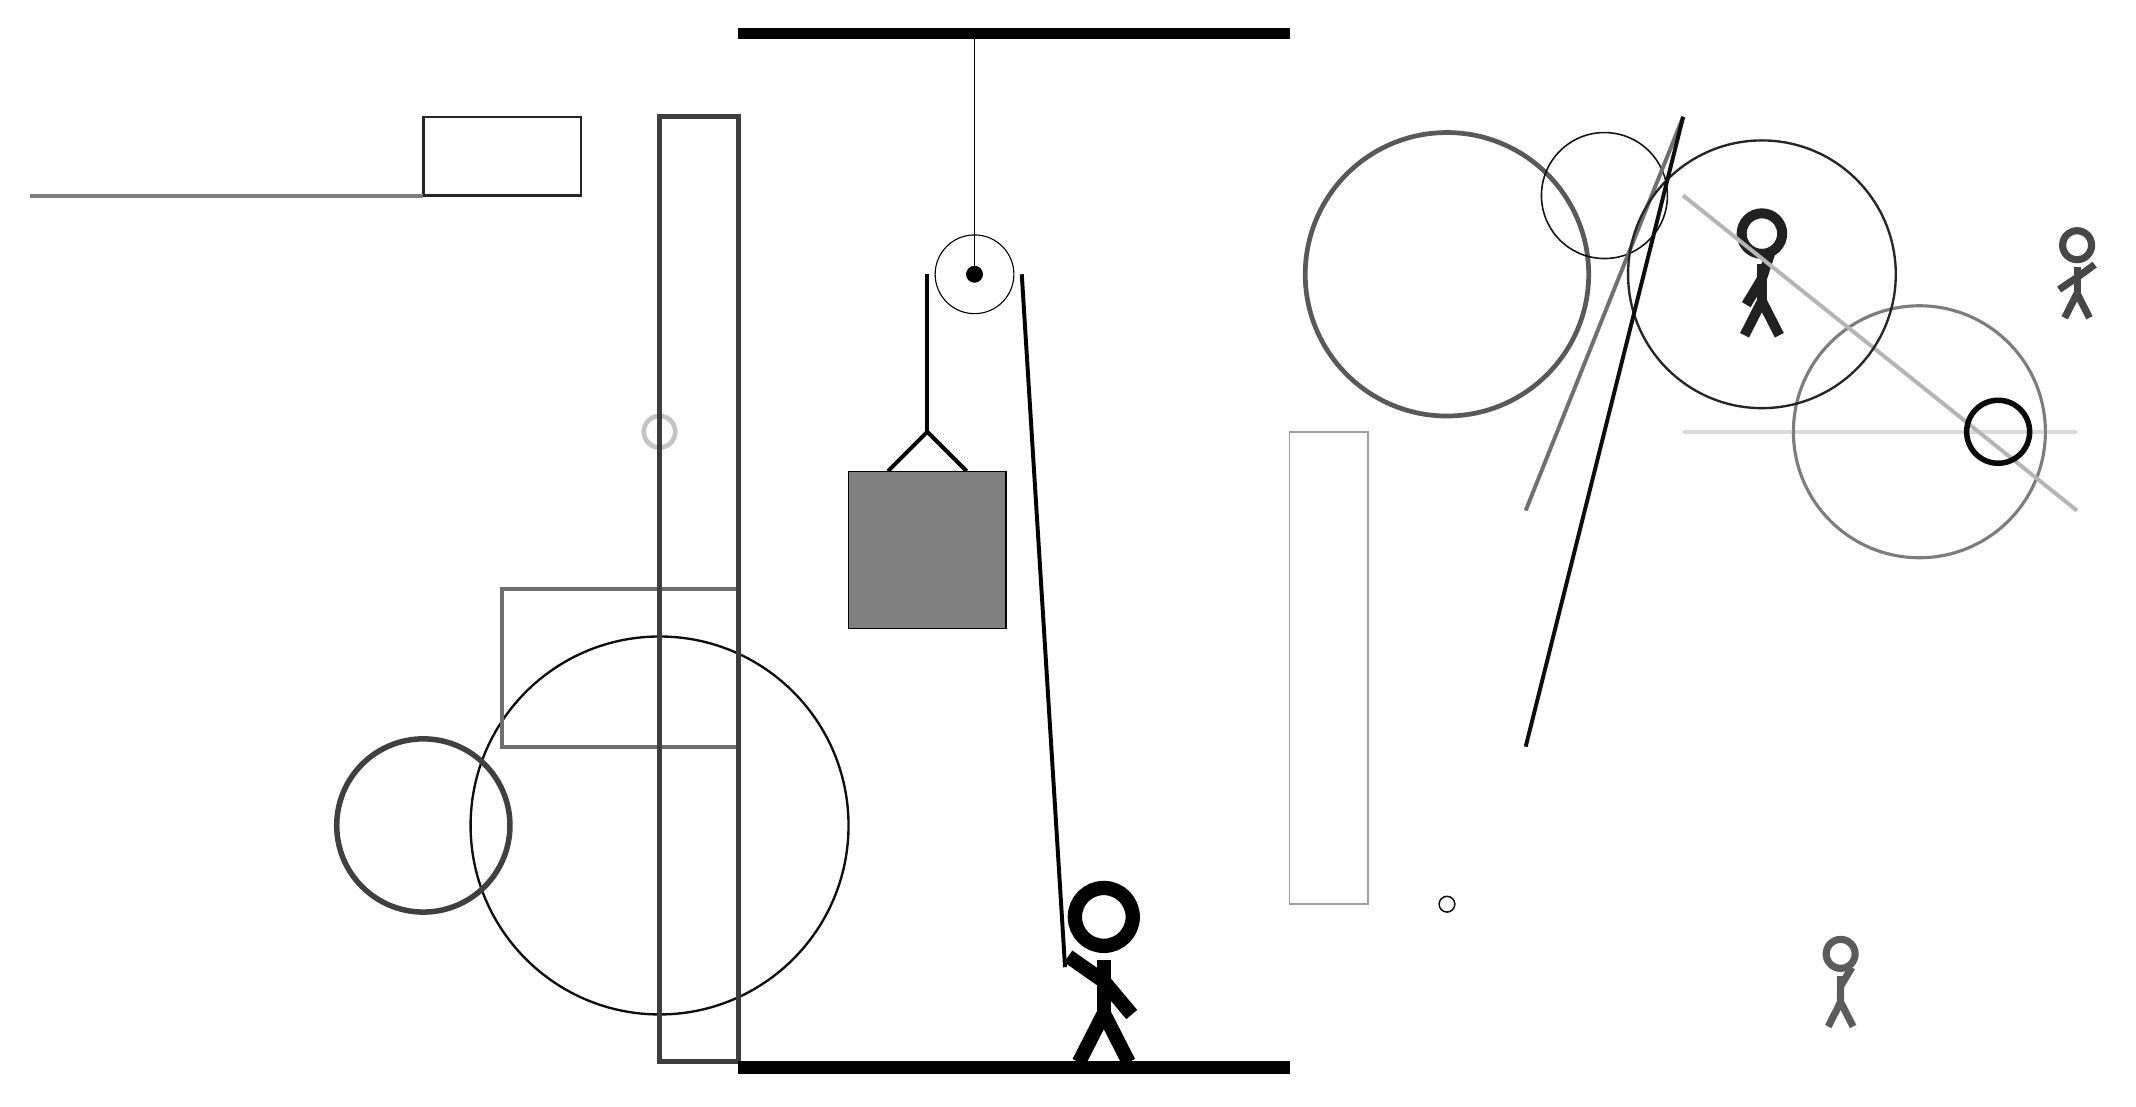
\begin{tikzpicture}
		%%%%% START %%%%%
		
		\draw[fill=black] (-2, 10) rectangle (5, 10.125);
		
		\draw[line width=0.5mm, color=black!14](10, 5) -- (15, 5);
		
		\draw[line width=0.2mm, color=black!38] (6, -1) rectangle (5, 5);
		\draw [line width=0.6mm, color=black!65](7, 7) circle (1.8);
		\draw[line width=0.3mm, color=black!85] (-4, 9) rectangle (-6, 8);
		\draw [line width=0.3mm, color=black!94](-3, 0) circle (2.4);
		\draw [line width=0.6mm, color=black!23](-3, 5) circle (0.2);
		
		\draw[line width=0.5mm, color=black!57] (-2, 1) rectangle (-5, 3);
		\node[line width=0.3mm, color=black!72] at (15, 7) {\Strichmaxerl[5][34][36]};
		\draw [line width=0.2mm, color=black!92](9, 8) circle (0.8);
		\node[line width=0.7mm, color=black!87] at (11, 7) {\Strichmaxerl[7][59][72]};
		\draw [line width=0.4mm, color=black!51](13, 5) circle (1.6);
		
		\draw[line width=0.6mm, color=black!76] (-2, 9) rectangle (-3, -3);
		\node[line width=0.7mm, color=black!64] at (12, -2) {\Strichmaxerl[5][89][59]};
		
		\draw [line width=0.7mm, color=black!75](-6, 0) circle (1.1);
		\draw[line width=0.5mm, color=black!29](10, 8) -- (15, 4);
		\draw [line width=0.4mm, color=black!18](6, -1) circle (0.0);
		
		\draw[line width=0.5mm, color=black!51](-6, 8) -- (-11, 8);
		
		\draw[line width=0.5mm, color=black!56](10, 9) -- (8, 4);
		\draw [line width=0.3mm, color=black!85](11, 7) circle (1.7);
		\draw [line width=0.2mm, color=black!92](7, -1) circle (0.1);
		\draw[line width=0.5mm, color=black!94](8, 1) -- (10, 9);
		
		\draw [line width=0.7mm, color=black!96](14, 5) circle (0.4);
		
		\draw (1, 7) circle (0.5);
		\draw[fill=black] (1, 7) circle (0.1);
		\draw (1, 10) -- (1, 7);
		
		\draw[line width=0.5mm] (-0.1, 4.5) -- (0.4, 5.0) -- (0.9, 4.5);
		\draw[fill=black!50] (-0.6, 4.5) rectangle (1.4, 2.5);
		
		\draw[line width=0.5mm] (0.4, 7) -- (0.4, 5.0);
		\centerarc[line width=0.5mm](1, 7)(0:180:0.6);
		\draw[line width=0.5mm](1.6, 7) -- (2.15, -1.8);
		
		\node at (2.6, -1.9) {\Strichmaxerl[10][-35][-50]};
		
		\draw[fill=black] (-2, -3) rectangle (5, -3.15);
		
		%%%%% END %%%%%
	\end{tikzpicture}
\end{document}